% Appendices (after the references in both builds). Generated content is never typed by hand: numbers are macros.
\appendix

\section{cuBLAS's batch-invariance mode on Blackwell}\label{app:blackwell}\label{sec:cublasmode}
cuBLAS 13.4 documents an experimental batch-invariance mode for compute capability 10.x, enabled per call or with the environment variable \texttt{CUBLAS\_BATCH\_INVARIANCE\_FLAGS}; it disables split-K and covers fp32, fp16, bf16, FP8 and FP4 \citep{nvidia2026cublas}. It is not in the cuBLAS release that vLLM pins. We loaded cuBLAS 13.8.2 in place of the pinned release and ran the bitwise test on a B200 with the mode set to automatic alignment, on \OneEShapes{} shape and dtype combinations: the router, the narrow shapes that fail on Hopper, odd widths, and large model shapes. Combined with the PyTorch settings that vLLM's batch-invariant mode applies (cuBLASLt preferred, reduced-precision reductions disabled), the mode does not pass our preregistered test: \OneEBadC{} of \OneECompC{} comparisons differ, all on odd output widths (\OneEBadShapesC{} shape and dtype combinations), with \OneEErrC{} errors; without the mode, on the same library, \OneEBadB{} differ across \OneEBadShapesB{}. With PyTorch's default settings, however, the mode is batch-invariant everywhere we looked: \OneEBadD{} of \OneECompD{} comparisons differ, including the router and every odd width, and in fp32 \OneEBadE{} of \OneECompE{}. The failure is therefore an interaction between the mode and vLLM's settings rather than a gap in the mode. We first suspected the automatic alignment setting, which the documentation says is invariant only if every call detects the same alignment class, but a diagnostic rules it out: forcing a fixed 2-byte class makes matters worse (\FAlignTwoBad{} of \FAutoComp{} comparisons differ, against \FAutoBad{} with automatic alignment), and a 16-byte class is rejected for odd widths (\FAlignSixteenErr{} errors). What breaks the mode is the reduced-precision setting through which vLLM disables split-K in PyTorch: with only cuBLASLt preferred and that setting left at its default, \FLtBad{} of \FLtComp{} comparisons differ on every shape. The mode already disables split-K, so the setting is redundant when the mode is on.

\section{Which shapes does cuBLAS compute batch-invariantly?}\label{app:shapes}
A finer sweep (Figure~\ref{fig:shapes}) shows that the boundary also depends on $K$ and on the cuBLAS workspace environment variables, which vLLM sets at runtime. With them, widths \NarrowNs{} are invariant at $K$ = \NarrowPassK{} but not at \NarrowFailK{}, and widths from \MidLo{} to \MidHi{} are invariant only when they are multiples of \MidMult{}. Without them, every tested width from \NoenvMinFailN{} to \NoenvMaxFailN{} fails at $K$ = \NoenvFailK{}, and only widths of \NoenvMinPassN{} or more pass at every $K$. An H200 gives the same result as the H100 on \HtwoAgree{} of \HtwoShapes{} shapes with the variables and \HtwoAgreeNoenv{} of \HtwoShapes{} without.

\begin{figure*}[t]\centering
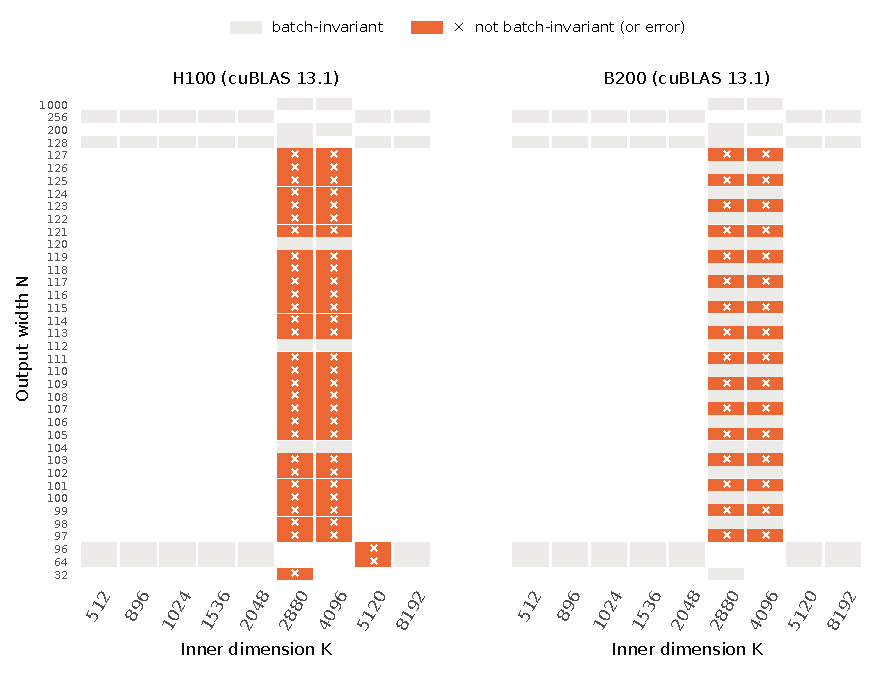
\includegraphics[width=0.95\linewidth]{fig_shapes.pdf}
\caption{Which matrix shapes cuBLAS computes batch-invariantly under batch-invariant mode's settings (batch sizes 1 to 1024, then every sixteenth to 8192; bf16 and fp16), on H100 and B200 with the same cuBLAS release. Blank cells were not tested. On B200 the bf16 cells marked for odd widths raise an error rather than differ.}\label{fig:shapes}
\end{figure*}

\section{gpt-oss: tuned configurations and breakable graphs}\label{app:gptoss}
At a maintainer's request, the upstream contribution covers shapes from widely used models instead: the bf16 layers of GLM-5.3 and DeepSeek-V4.1 that reach this kernel under batch invariance (routers, sparse-attention indexer projections, DeepSeek-V4.1's compressor and \texttt{lm\_head} per tensor-parallel rank; the rest of both models is FP8 or FP4 and uses other kernels), and gpt-oss's attention, routers and \texttt{lm\_head}. Over all \PopShapes{} shapes, \PopBad{} of \PopRows{} rows differ in the bitwise check, and the tuned kernels are \PopSpeedMin{}--\PopSpeedMax{}$\times$ faster than the default at every bucket. End to end the gain is small, because most of these models' computation runs in quantized expert kernels that the table does not touch: decode-heavy serving throughput rises by \OssGain{} for gpt-oss-20b and \OssBigGain{} for gpt-oss-120b, faster in \OssWins{} and \OssBigWins{} of \OssRounds{} rounds; for gpt-oss-20b the loss against the mode off falls from \OssStockLoss{} to \OssTunedLoss{}. Tuning pays off in proportion to the share of a model's computation in unquantized Linear layers: dense bf16 models gain the most.

On the PR branch build, forcing breakable CUDA graphs changes the gpt-oss-20b decode-heavy comparison from a \GptossNoBreakDecGain{} gain over stock to \GptossBreakDecGain{}; the branch wins \GptossBreakDecWins{} of \GptossBreakRounds{} rounds. On the prefill-heavy workload, its mean difference from stock changes from \GptossNoBreakPreGain{} to \GptossBreakPreGain{}, with \GptossBreakPreWins{} wins in the rerun. That prefill loss without breakable graphs was measured at the branch's merge base; an independent maintainer measurement on a later vLLM main, on H100 and H200 with three rounds, did not reproduce it \citep{vllm65931}, so we do not treat it as a property of the configurations. The effect is consistent with the graph lookup mechanism: the config table chooses tiles by runtime batch size, and a compiled forward can retain the choice made during capture. Breakable graphs preserve the per-batch lookup. vLLM's automatic batch-invariant path excludes models with quantization enabled, including gpt-oss, even though the measured BF16 projections use the tuned table. These two rerun rounds are evidence for the decode mechanism; they are not a precision estimate. A follow-up change that lets the automatic path include MXFP4 models, whose dense Linear layers stay bf16, confirms the mechanism on a current vLLM main with \OssGateRounds{} rounds on each of H100 and H200: against the merged configurations alone, it raises gpt-oss-20b single-request decode throughput by \OssGateDecOneMin{}--\OssGateDecOneMax{} and concurrency-32 decode by \OssGateDecMin{}--\OssGateDecMax{} (faster in every round), while the prefill-heavy median stays within \OssGatePreAbsMax{}.

\section{Serving-cost and implementation evidence}\label{app:serving}
\subsection{Where the cost comes from}\label{sec:cost}
The default configuration uses 128-row tiles at every batch size. At decode batch sizes most of each tile is padding, so the kernel does several times the necessary work. Tuned entries choose small tiles for small batches. This explains the spread above: the models with tuned entries lose \LlamaStock{} and \QthreeStock{}, the untuned ones \QsevenStock{} and \GemmaStock{}. The tile lookup depends on runtime batch size, but torch.compile can capture a single lookup result in the compiled forward. vLLM uses breakable CUDA graphs to keep that lookup tied to the runtime batch size for eligible tuned models; its automatic path excludes quantized model configurations, even when an unquantized projection in the model has a tuned entry. Appendix~\ref{sec:tune} and Appendix~\ref{app:gptoss} measure the effect of this exclusion.



\subsection{Route 1: tune the Triton kernel}\label{sec:tune}
We tuned the five Qwen2.5-7B Linear shapes in vLLM's table format: for each shape one \texttt{BLOCK\_K} (64 or 128), and per batch-size bucket the fastest tile sizes, warp count and pipeline depth, chosen by timing on an H100. The tuned kernels run \TuneSpeedMin{}--\TuneSpeedMax{}$\times$ faster than the default at batch sizes up to 32, within \TuneSmallMin{}--\TuneSmallMax{}$\times$ of cuBLAS there, and \TuneLargeMin{}--\TuneLargeMax{}$\times$ slower than cuBLAS on the attention and MLP projections at batch sizes of 256 and more.

Invariance is unchanged: \TuneBad{} of \TuneRows{} rows differ between a row alone and inside batches of 1 to 8192 rows, over all \TuneShapes{} shapes, and with the table loaded in vLLM \TuneCrossMis{} of \TuneCrossReq{} requests change across serving conditions. In the three-repeat rerun, decode loss falls from \TuneStockMin{}--\TuneStockMax{} to \TuneLossMin{}--\TuneLossMax{} across batch sizes up to \TuneBmax{} (Figure~\ref{fig:cost}, Table~\ref{tab:tune}); at batch 32 it is \TunedB{} against \TuneStockB{}. Our preregistered target was at most 5\%, so tuning alone does not close the whole gap; what remains is the kernel's speed at larger batch sizes, which a faster batch-invariant matrix-multiplication kernel would address.

\begin{figure}[t]\centering
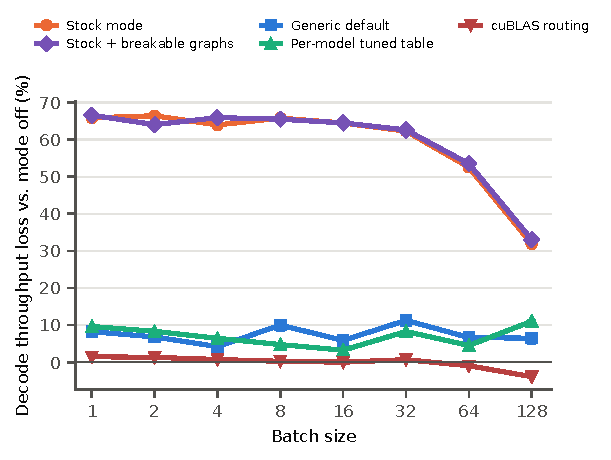
\includegraphics[width=0.75\linewidth]{fig_cost.pdf}
\caption{Qwen2.5-7B decode throughput loss against batch-invariant mode off on H100, by batch size. For the four rerun arms, markers show the ratio of arm medians and whiskers span the paired per-run loss range; whiskers are descriptive, not confidence intervals. The cuBLAS curve is from the separate main cost measurement (Appendix~\ref{sec:cublas}).}\label{fig:cost}
\end{figure}

\begin{table*}[t]\centering\small
% Generated by src/make_macros.py from results/stats.json; each row is checked against results/generic2 run records.
\begin{tabular}{lrrrrrrrr}
\toprule
Batch size & 1 & 2 & 4 & 8 & 16 & 32 & 64 & 128 \\
\midrule
Stock mode (default config) & 65.9\% & 66.4\% & 63.9\% & 65.8\% & 64.5\% & 62.3\% & 52.5\% & 31.9\% \\
Stock + breakable & 66.6\% & 64.0\% & 65.9\% & 65.5\% & 64.5\% & 62.6\% & 53.5\% & 33.0\% \\
Generic + breakable & 8.2\% & 6.8\% & 4.2\% & 10.0\% & 5.9\% & 11.3\% & 6.7\% & 6.5\% \\
Per-model tuned table & 9.6\% & 8.3\% & 6.4\% & 4.8\% & 3.2\% & 8.3\% & 4.5\% & 11.0\% \\
\bottomrule
\end{tabular}

\caption{Qwen2.5-7B decode throughput loss against batch-invariant mode off on H100. All four batch-invariant arms use medians of three jobs from the better-default rerun.}\label{tab:tune}
\end{table*}

\paragraph{Serving benchmark and upstream contribution.} In an online serving benchmark (\texttt{vllm bench serve}, random prompts, concurrency 32, fresh server per run), the tuned table raised decode-heavy output throughput by \ServeDecGain{} over stock mode, winning \ServeWins{} of \ServeRounds{} alternating rounds; the loss against the mode off fell from \ServeDecStockLoss{} to \ServeDecTunedLoss{}. On a prefill-heavy workload the gain was \ServePreGain{}. \ifanon The configurations were contributed to vLLM\else We contributed the configurations to vLLM\fi{} in the format of earlier tuned-table contributions \citep{vllm62219,vllm65903}, with a unit test that checks configuration selection and exact output equality on both sides of every bucket boundary (\ServeUnit{} tests pass) \citep{vllm65931}.

\paragraph{Popular models.} At a maintainer's request, the upstream contribution covers bf16 layers of GLM-5.3, DeepSeek-V4.1 and gpt-oss instead; the kernels are \PopSpeedMin{}--\PopSpeedMax{}$\times$ faster than the default, with \PopBad{} of \PopRows{} rows differing, but end-to-end gains are small because most of these models' computation runs in quantized expert kernels (Appendix~\ref{app:gptoss}).

\paragraph{Breakable graphs for quantized models.} The same lookup effect limits gpt-oss: vLLM's automatic breakable-graph path excludes quantized models even when their bf16 projections use the tuned table. Letting it include MXFP4 models raises gpt-oss-20b single-request decode throughput by \OssGateDecOneMin{}--\OssGateDecOneMax{} on H100 and H200, with prefill unchanged (Appendix~\ref{app:gptoss}).



\subsection{Route 3: route Linear layers to cuBLAS}\label{sec:cublas}
\paragraph{Is cuBLAS batch-invariant?} We multiply each row alone and inside batches of 1 to 8192 rows, at every Linear shape of six models, in bf16 and fp16, and compare rows near the start and end of the batch (Table~\ref{tab:bitwise}). Under batch-invariant mode's settings, no row differed on any of \PoneBuildsHundred{} H100 builds or \PoneBuildsBlackwell{} B200 builds (\PoneCublasVersions{} cuBLAS versions; \PoneBadTotal{} of \PoneComparisons{} comparisons), including with a second process saturating the GPU. With PyTorch defaults, between \PoneCtlMinH{} and \PoneCtlMaxH{} of \PoneRowsPerMode{} rows differed on H100, and \PoneCtlB{} on B200, so the test detects batch dependence when it exists.

\begin{table*}[t]\centering\small
% Generated by src/make_macros.py. Do not edit.
\begin{tabular}{lrrr}
\toprule
GPU, torch build & BI flags & Flags only & Defaults \\
\midrule
B200, torch t2.13.0+cu130 & 0 & 0 & 19{,}544 \\
B200, torch t2.14.0+cu130 & 0 & 0 & 19{,}544 \\
H100, torch t2.11.0+cu128 & 0 & 0 & 7{,}344 \\
H100, torch t2.12.0+cu126 & 0 & 0 & 6{,}784 \\
H100, torch t2.13.0+cu126 & 0 & 0 & 6{,}784 \\
H100, torch t2.13.0+cu129 & 0 & 0 & 7{,}344 \\
H100, torch t2.13.0+cu130 & 0 & 0 & 8{,}544 \\
H100, torch t2.14.0+cu126 & 0 & 0 & 6{,}784 \\
H100, torch t2.14.0+cu130 & 0 & 0 & 8{,}544 \\
H100, torch t2.14.0+cu130 + GPU load & 0 & 0 & 8{,}544 \\
\bottomrule
\end{tabular}

\caption{Rows that differ between a row multiplied alone and inside a batch, out of \PoneRowsPerMode{} per cell. BI flags: environment variables and PyTorch flags as batch-invariant mode sets them. Flags only: PyTorch flags without the cuBLAS environment variables. Defaults: PyTorch defaults (control).}\label{tab:bitwise}
\end{table*}

\paragraph{Which shapes?} A denser test checked every batch size from 1 to 1024 and every sixteenth up to 8192, on \ShapeCount{} shapes including mixture-of-experts routers and a sweep of narrow output widths $N$. On H100, at $K = 2880$ and $4096$, every shape with $N \le \ShapeMaxFailN{}$ is batch-variant under the mode's settings, and every shape with $N \ge \ShapeMinPassN{}$ is batch-invariant at every batch size. The boundary also depends on $K$, on the cuBLAS workspace environment variables and on the GPU (Appendix~\ref{app:shapes}). The gpt-oss-20b router ($N=32$, $K=2880$) diverges from batch size \RouterBfFirstBad{} in bf16 and \RouterFpFirstBad{} in fp16, and on H200 its failures are interleaved with passing batch sizes \citep{vllm65569}, so a check that samples a few batch sizes at model load could pass a shape that fails at others.

\paragraph{Serving determinism and cost.} With Linear layers on cuBLAS, \PtwoPassConfigs{} of \PtwoConfigs{} serving configurations produced identical tokens and top-$k$ logprobs across all conditions (Table~\ref{tab:det}); controls with the mode off diverged on \PtwoCtlDivMin{} to \PtwoCtlDivMax{} of requests. The exception, Gemma-2-9B, fails under vLLM's own mode too (Appendix~\ref{sec:gemma}). Decode loss at batch 32 falls to \QsevenPlain{} for Qwen2.5-7B and \GemmaPlain{} for Gemma-2-9B (Table~\ref{tab:cost}); \PtwoCostPass{} of \PtwoCostCells{} measured cells meet our preregistered 5\% limit. At two-way tensor parallelism the residual loss (\TwoPPlain{}) comes from the mode's fixed-order communication, which costs \TwoPComm{} on its own. Routing only shapes that pass a load-time check, so that routers stay on the Triton kernel, keeps gpt-oss-20b's batch-invariance tests passing (\GptossVtwoPass{} of \GptossTests{}, the same as stock mode's \GptossOnPass{}), while routing every Linear layer fails all of them (\GptossBlanketPass{} of \GptossTests{} pass), reproducing the failure that motivated the Triton default \citep{vllm35404}.

\begin{table*}[t]\centering\small
% Generated by src/make_macros.py. Do not edit.
\begin{tabular}{lrrr}
\toprule
Configuration & Plain cuBLAS & Mode off & Markers \\
\midrule
Qwen2.5-7B, TP=2 & 0 / 100 & 38 / 100 & 2 \\
Qwen2.5-7B, TP=4 (TP=2 control) & 0 / 100 & 38 / 100 & 4 \\
Qwen2.5-7B, long context, chunked prefill & 0 / 50 & 29 / 50 & 1 \\
Qwen2.5-7B, seeded sampling & 0 / 100 & 40 / 100 & 1 \\
Qwen2.5-32B, TP=2 & 0 / 100 & 76 / 100 & 2 \\
Mistral-7B & 0 / 100 & 4 / 100 & 1 \\
Gemma-2-9B & 39 / 100 & 60 / 100 & 1 \\
\bottomrule
\end{tabular}

\caption{Requests whose 8 runs were not all identical, with Linear layers on cuBLAS under batch-invariant mode (plain cuBLAS) and with batch-invariant mode off (control). Markers count processes that loaded the routing change.}\label{tab:det}
\end{table*}

\begin{table*}[t]\centering\small
% Generated by src/make_macros.py. Do not edit.
\begin{tabular}{lrrr}
\toprule
Model & Stock & Plain cuBLAS & Plain, worst repeat \\
\midrule
Qwen2.5-7B & 63.1\% & 0.2\% & 3.1\% \\
Gemma-2-9B & 59.2\% & 1.0\% & 1.3\% \\
Mistral-7B & 5.8\% & 3.3\% & 5.9\% \\
Qwen2.5-7B, TP=2 & 61.0\% & 5.8\% & 6.8\% \\
Qwen2.5-32B, TP=2 & 58.2\% & $-$2.3\% & $-$1.0\% \\
\bottomrule
\end{tabular}

\caption{Decode throughput loss at batch 32 against batch-invariant mode off. Median of three jobs.}\label{tab:cost}
\end{table*}

\paragraph{Why we do not recommend it.} cuBLAS is the cheapest route measured, but NVIDIA does not document its default kernels as batch-invariant, and the boundary we observe moves with $K$, with when the environment variables reach cuBLAS, and across batch sizes. The boundary is also GPU-specific: on a B200 with the same cuBLAS release, the failing shapes are exactly the odd widths from \BtwoFailMin{} to \BtwoFailMax{}, the router passes, and \BtwoDiffer{} of \BtwoShapes{} shapes have a different result than on H100. For bf16 odd widths the batch-invariant settings fail outright on B200: cuBLASLt rejects the shape and PyTorch's fallback refuses the split-K setting (\OneEErrA{} shapes in the Blackwell sweep). An upstream change would have to rest on a property that a library update could silently remove.



\subsection{A serving-level failure: Gemma-2}\label{sec:gemma}
Gemma-2-9B is not batch-invariant under vLLM's batch-invariant mode on H100: \GemmaOnDiv{} of \GemmaReq{} requests diverged with stock mode (\GemmaPlainDiv{} with cuBLAS routing, \GemmaOffDiv{} with the mode off). Varying one component at a time (\DiagReq{} requests each) localizes it: switching attention to the Triton backend removes it (\DiagTritonOn{} diverging, control \DiagTritonOff{}), as does eager execution (\DiagEagerOn{}, control \DiagEagerOff{}), disabling the sliding window (\DiagNoswOn{}, control \DiagNoswOff{}), or turning off CUDA graphs while keeping compilation (\DiagNocgOn{}, control \DiagNocgOff{}); removing logit softcapping does not (\DiagNoscOn{}, control \DiagNoscOff{}). \ifanon The failure was reported upstream; a contributor\else We reported this upstream; another contributor\fi{} traced it to FlashAttention~3 dropping the sliding window when the window covers the batch's longest sequence, which changes the key-value tile between captured CUDA graphs and eager steps, and fixed it by keeping the window active under batch invariance, a change that has since been merged \citep{vllm65627}. On our H100 the issue's reproducer goes from \FafixBase{} of \FafixN{} prompts differing between alone and batched to \FafixFix{} of \FafixN{} with the fix.
